\documentclass{article}
\usepackage{listings}
\usepackage{mathrsfs}
\usepackage[utf8]{inputenc}
\usepackage{amssymb}
\usepackage{lipsum}
\usepackage{amsmath}
\usepackage{fancyhdr}
\usepackage{geometry}
\usepackage{scrextend}
\usepackage[english,german]{babel}
\usepackage{titling}
\setlength{\droptitle}{-3cm}
\usepackage{tikz}
\usepackage{algorithm,algpseudocode}
\usepackage[doublespacing]{setspace}
\usetikzlibrary{datavisualization}
\usetikzlibrary{datavisualization.formats.functions}
\usepackage{polynom}
\usepackage{amsmath}
\usepackage{gauss}
\usepackage{tkz-euclide}
\usetikzlibrary{datavisualization}
\usetikzlibrary{datavisualization.formats.functions}
\author{
Alexander Mattick Kennung: qi69dube\\
Kapitel 1
}
\usepackage{import}
\date{\today}
\geometry{a4paper, margin=2cm}
\usepackage{stackengine}
\parskip 1em
\newcommand\stackequal[2]{%
  \mathrel{\stackunder[2pt]{\stackon[4pt]{=}{$\scriptscriptstyle#1$}}{%
  $\scriptscriptstyle#2$}}
 }
\makeatletter
\renewcommand*\env@matrix[1][*\c@MaxMatrixCols c]{%
  \hskip -\arraycolsep
  \let\@ifnextchar\new@ifnextchar
  \array{#1}}
\makeatother
\lstset{
  language=haskell,
}
\lstnewenvironment{code}{\lstset{language=Haskell,basicstyle=\small}}{}
\usepackage{enumitem}
\setlist{nosep}
\usepackage{titlesec}

\titlespacing*{\subsection}{0pt}{2pt}{3pt}
\titlespacing*{\section}{0pt}{0pt}{5pt}
\titlespacing*{\subsubsection}{0pt}{1pt}{2pt}
\title{Vorlesung 6}


\begin{document}
	\maketitle
	\section{Wahrscheinlichkeitsdichte und Verteilungsfunktion}
	Ziel $A\in\mathcal{A}: P(A)=?$\\
	$\to$ Wahrscheinlichkeitsdichte und Verteilungsfunktion.\\
	Skalieren eines histograms auf relative häufigkeiten: $\sum\limits^n_{k=0} h_n(k)=1$\\
	$\Omega =\{1,\dots,n\}$ $P(\{i\})=\frac{1}{n}$
	$\Omega$ sei eine abzählbare Ergebnismenge und $\mathcal{A}=\mathcal{P}(\Omega)$\\
	1. Ist P ein W-Maß über $(\Omega,\mathcal{A})$ und $f(\omega)=P(\{\omega\})$\\
	\[f(\omega)\geq 0, \sum\limits_{\omega\in\Omega} f(\omega)=1\]
	\[P(A)=\sum\limits_{\omega\in A}f(\omega),\ (A\in\mathcal{A})\]
	Jede Abbildung $f:\Omega\to \mathbb{R}$ mit den beiden Eigneschaften ist ein W-Maß auf P mit eigenschaft
	\[P(\{\omega\})=f(\omega)\]
	die Abbildung f heißt Zähldichte (Z-Dichte)
	was ist mit kontinuirlichen Verteilung über z.B. $\mathbb{N}$?\\
	$f(\omega)\geq 0\forall \omega\in\Omega$\\
	$f:\mathbb{N}\to \mathbb{R}^+_0$\\
	$P(\Omega)=P(\mathbb{N})=P(\sum\limits^\infty_{k=1}\{k\})=\sum\limits^\infty_{k=1}P(\{k\})$\\
	Ein Beispiel wäre $f(k)=cq^k$ mit $q\in(0,1)$, $c\in\mathbb{R}$\\
	i) $P(A)\geq 0,\forall A\in\mathcal{A}$ ii) nichtnegativität $P(\Omega)=1$ normiertheit iii) sigma-additivität\\
	\textbf{Binomialverteilung}\\
	Sei $p+q=1, p,q\in\mathbb{R}$ und $\Omega = \{0,1,\dots, n\}$
	\[f(k)=b(n,p;k)=\binom{n}{k} p^kq^{n-k}\]
	wobei der graph über k läuft und n/p nur parameter sind.\\
	Beweis:\\
	$P(\{k\})\geq 0$
	$P(\Omega) = \sum\limits^n_{k=0}f(k) = \sum\limits^n_{k=0}\binom{n}{k}p^kq^{n-k}=(p+q)^n=1^n=1$\\
	additivität folgt aus der Verlauf über $\mathbb{R}$\\
	$A\to h_n(A) = \frac{1}{n} \text{Anzahl x mit} x\in A$\\
	Zähldichte der \textbf{empirische Verteilung} von x\\
	\[f_n^x = \frac{1}{n} \sum\limits^n_{i=1} 1_{x_i}(x)\ x\in\Omega\]
	$\to$ diskretes Rieman-Integral.\\
	Stetige Dicht:\\
	Eine Riemann-integrierbare Funktion $f:\mathbb{R}\to\mathbb{R}$ mit\\
	\[\forall x.f(x)\geq 0\text{ und }\int\limits^\infty_{-\infty} f(x)dx =1\]
	heißt \textbf{Riemann-Dichte} über $\mathbb{R}$ oder auch \textbf{stetige Dichte}.\\
	Jeder R-Dichte über $\mathbb{R}$ definiert eindeutig ein W-Maß p über $(\mathbb{R},\mathbb{B})$ mit der Eigenschaft
	\[P((a,b])=P([a,b])=\int\limits^b_a f(x)dx\]
	mit $a\leq b$ und $P(\{\omega\})=0$\\
	Fortsetzungssatz:\\
	Ist P auf einem geeigneten erzeuger $\varepsilon$ von $\mathcal{A}$ festgelegt und auf $\varepsilon$ nicht-negativ, sigma-additiv und normiert, kann man sie eindeutig auf P von $\mathcal{A}$ fortsetzen.\\
	\textbf{Empirische Verteilungsfunktion}\\
	$\hat F^x_n:= \frac{1}{n} \sum\limits^n_{i=1} 1_{[x_i,\infty)} (x),\ x\in\mathbb{R}$\\
	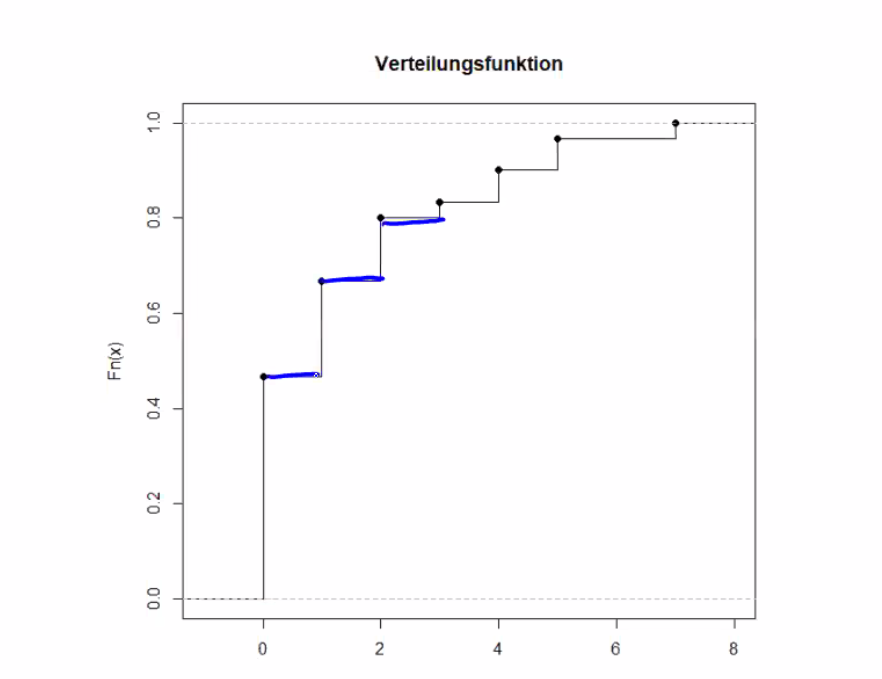
\includegraphics[height=128px]{verteilungsfunktion.png}\\
	Eine Wahrscheinlichkeitsdichtefunktion muss nicht stetig sein $f(x)=\begin{cases}0&x\leq a\\ (b-1)&x\leq b\\0&x\geq b\\\end{cases}$\\
	Diese kann stetig gemacht werden, indem man den integral der Riemann-Dichte integriert:\\
	\[P([a,b])=\int^a_b f(t)dt\]
	also ist 
	\[F(x)=\int^x_{\infty} f(t) dt\]
	\begin{tabular}{|c|c|}\hline
	$\Omega$-abzählbar&$\Omega$-kont\\\hline
	$P(\{\omega\})=f(\omega)$& $f(x)\geq 0$, $\int^fd\tau=1$\\
	$P(A)=\sum_{\omega\in A}f(\omega)$&$P((a,b])=\int^b_afd\tau$\\
	Z-dichte&R-dichte\\\hline
	\end{tabular}\\
	Ist F die VF (verteilungsfunktion) eines W-Maßes P über $(\mathbb{R},\mathbb{B})$, dann gilt:\\
	\begin{itemize}
		\item F ist isoton, d.h. monoton nicht fallend (entweder steigend, oder konstant)
		\item F ist ``normiert'', d.h. die grenzwerte sind 0 und $\infty$
		\item F ist rechtsseitig stetig
		\item F besitzt einen linksseitigen Grenzwert $F(x-) = \lim\limits_{h\to 0^+} F(x-h)=P((-\infty,x))$
		\item Für Einpunktmengen $\{x\}$ gilt: $P(\{x\})=F(x)-F(x-)$
	\end{itemize}
\end{document}